\documentclass[11pt]{article}
\usepackage[a4paper, margin=2.5cm]{geometry}
\usepackage{amsmath}
\usepackage{amssymb}
\usepackage{graphicx}
\usepackage{booktabs}
\usepackage{siunitx}
\usepackage{hyperref}
\usepackage{float}
\usepackage{longtable}
\usepackage{caption}
\usepackage[authoryear]{natbib}
\graphicspath{{figures/}}
\title{Estimating the Hubble Constant: \\ From Historical to Modern Data}
\author{Alessandro Buttazzo \\ \small [Nome del Liceo], Milano \\ \small Independent research project, not conducted within a formal school or institutional research program}
\date{August 2, 2026}
\begin{document}
\maketitle
\tableofcontents
\newpage
\begin{abstract}
This project estimates the Hubble constant $H_0$ using two independent datasets: Edwin Hubble's original 1929 sample of 24 extragalactic objects, and a modern sample of 37 galaxies with distances and redshifts drawn from the NASA/IPAC Extragalactic Database (NED). By comparing historical and modern results, the project examines how limitations in the extragalactic distance scale of the 1920s led to a significant overestimate of the expansion rate of the Universe, and situates both results against the values reported by current large-scale surveys. Beyond reproducing the headline numbers, statistical uncertainties are attached to every fit, and a jackknife/bootstrap sensitivity analysis quantifies how much the modern result depends on the five most distant (maser) galaxies in the sample, showing that no single object drives the result even though the group as a whole is essential to reaching agreement with the accepted value. An inverse-variance weighted fit is also attempted, combining representative distance-method uncertainties with a peculiar-velocity scatter floor; this both illustrates a common pitfall (naively weighting by distance precision alone reintroduces the very peculiar-motion bias the sample extension was designed to suppress) and yields a more conservative, better-motivated error budget, which is compared directly against Planck, SH0ES, and TRGB measurements. A further check using orthogonal distance regression, which accounts for measurement error on distance as well as velocity, shifts the estimate upward again, underlining that the exact point estimate is less robust than any single fit alone would suggest.
\end{abstract}
\section{Introduction}
Hubble's Law is one of the foundational results of modern cosmology: it provided the first empirical evidence that the Universe is expanding, and remains central to how astronomers measure cosmic distances, ages, and the overall scale of the Universe. The value of the Hubble constant $H_0$ sets the present-day expansion rate of the Universe and is directly linked to its estimated age: a higher $H_0$ implies a younger Universe, and vice versa.
Hubble's Law states that the recession velocity $v$ of a galaxy is proportional to its distance $r$ from us:
\begin{equation}
v = H_0 \, r
\label{eq:hubble_law}
\end{equation}
where $H_0$ is the Hubble constant, typically expressed in km/s/Mpc.

It is worth being explicit about what Equation~\ref{eq:hubble_law} actually is: the leading-order (linear) term of a Taylor expansion of the cosmic scale factor $a(t)$ around the present time, valid only for redshifts $z \ll 1$. Writing the expansion one order further introduces the deceleration parameter $q_0$, so that the distance-redshift relation gains a quadratic correction, $cz \approx H_0 r \left[1 + \tfrac{1}{2}(1-q_0)\,\tfrac{H_0 r}{c} + \dots\right]$, which becomes relevant only once recession velocities are a non-negligible fraction of the speed of light. Every object in both samples used here has $v \ll c$ (at most about 3.4\% of $c$ for the most distant maser galaxy, NGC 6264, at $v\approx10{,}145$ km/s), so the linear, single-parameter form used throughout this project is an excellent approximation, and no attempt is made to constrain $q_0$ or any higher-order cosmological parameter from this data.

This project revisits the very first measurement of $H_0$, published by Edwin Hubble in 1929 \citep{hubble1929}, and compares it with a modern estimate obtained using the same statistical method but with contemporary distance measurements. The goal is not simply to reproduce a historical number, but to understand \emph{why} Hubble's original estimate differed so substantially from the value accepted today, and what this reveals about the evolution of observational astronomy over the past century. Hubble's own initial value, $H_0 \approx 500$ km/s/Mpc, was already revised upward within a few years, and in 1935 Arthur Eddington, combining relativity and quantum theory, confidently claimed to have found "a solution which I regard as definitive," with $H_0 = 865$ km/s/Mpc \citep{tully2023} --- a reminder that overconfidence in a single method has a long history in this field, one this project tries to avoid by explicitly comparing two independent approaches, attaching uncertainties to every result, and being transparent about their respective limitations.
Despite nearly a hundred years of increasingly precise measurements, the exact value of $H_0$ remains a subject of active debate. Measurements based on the local Universe --- using distance-ladder methods such as Cepheids and Type Ia supernovae --- give $H_0 = 73.3 \pm 1.0$ km/s/Mpc \citep{riess2022}, while measurements inferred from the cosmic microwave background under the standard $\Lambda$CDM model give $H_0 = 67.4 \pm 0.5$ km/s/Mpc \citep{planck2020}. A third, largely independent local method, based on the Tip of the Red Giant Branch (TRGB), gives an intermediate value of $H_0 = 69.8 \pm 0.6\text{ (stat)} \pm 1.6\text{ (sys)}$ km/s/Mpc \citep{freedman2021}, consistent with both the CMB value and, within its larger systematic uncertainty, the Cepheid-based value. This discrepancy between the Cepheid and CMB values, known as the \emph{Hubble tension}, now exceeds 5$\sigma$ significance --- meaning the probability that it is merely a statistical fluctuation is less than about 1 in 3.5 million --- and has persisted despite improved instrumentation, including cross-checks with the James Webb Space Telescope, suggesting it may point to genuinely new physics rather than a systematic measurement error. While a full treatment of this tension is beyond the scope of this project, it highlights that the precise determination of $H_0$ remains an open problem at the forefront of astrophysics --- one to which this project's own two estimates, despite their modest scale, can be meaningfully compared.
\section{Part 1: Reproducing Hubble's Original Analysis (1929)}
\subsection{Data and Method}
I used the original dataset published by Hubble (1929), consisting of 24 extragalactic objects with measured distance $r$ (in megaparsecs) and radial velocity $v$ (in km/s). To estimate the Hubble constant, I performed a linear fit of the form $v = H_0r$, using two approaches: an unconstrained linear regression (allowing a free intercept) and a regression forced through the origin, which is the physically motivated form of Hubble's Law, since a galaxy at zero distance should show zero recession velocity due to cosmic expansion. For every fit, I also report the standard error on $H_0$ from ordinary least squares and the coefficient of determination $R^2$, to quantify both the precision and the quality of the fit.
Table~\ref{tab:hubble1929_data} reports the full dataset used, taken directly from Hubble's original 1929 paper: distance $r$ (in Mpc) and radial velocity $v$ (in km/s) for each of the 24 objects in the sample.
{\small
\renewcommand{\arraystretch}{0.8}
\begin{longtable}{lcc}
\toprule
Object & $r$ (Mpc) & $v$ (km/s) \\
\midrule
\endfirsthead
\toprule
Object & $r$ (Mpc) & $v$ (km/s) \\
\midrule
\endhead
\bottomrule
\endfoot
\bottomrule
\endlastfoot
S. Mag. & 0.032 & +170 \\
L. Mag. & 0.034 & +290 \\
N.G.C. 6822 & 0.214 & $-$130 \\
N.G.C. 598 & 0.263 & $-$70 \\
N.G.C. 221 & 0.275 & $-$185 \\
N.G.C. 224 & 0.275 & $-$220 \\
N.G.C. 5457 & 0.45 & +200 \\
N.G.C. 4736 & 0.5 & +290 \\
N.G.C. 5194 & 0.5 & +270 \\
N.G.C. 4449 & 0.63 & +200 \\
N.G.C. 4214 & 0.8 & +300 \\
N.G.C. 3031 & 0.9 & $-$30 \\
N.G.C. 3627 & 0.9 & +650 \\
N.G.C. 4826 & 0.9 & +150 \\
N.G.C. 5236 & 0.9 & +500 \\
N.G.C. 1068 & 1.0 & +920 \\
N.G.C. 5055 & 1.1 & +450 \\
N.G.C. 7331 & 1.1 & +500 \\
N.G.C. 4258 & 1.4 & +500 \\
N.G.C. 4151 & 1.7 & +960 \\
N.G.C. 4382 & 2.0 & +500 \\
N.G.C. 4472 & 2.0 & +850 \\
N.G.C. 4486 & 2.0 & +800 \\
N.G.C. 4649 & 2.0 & +1090 \\
\caption{Distance and radial velocity data for the 24 objects in Hubble's (1929) sample.}
\label{tab:hubble1929_data} \\
\end{longtable}
}
\subsection{Results}
\begin{center}
\begin{tabular}{lcc}
\toprule
Sample & Free intercept (km/s/Mpc) & Forced through origin (km/s/Mpc) \\
\midrule
Full sample (24 galaxies) & $454 \pm 75$ \ ($R^2=0.62$) & $424 \pm 42$ \ ($R^2=0.62$) \\
Excluding Local Group (18 galaxies) & $409 \pm 98$ \ ($R^2=0.52$) & $433 \pm 41$ \ ($R^2=0.52$) \\
\bottomrule
\end{tabular}
\captionof{table}{Estimated $H_0$ from Hubble's 1929 data under different fitting assumptions, with standard errors and $R^2$ from ordinary least squares.}
\label{tab:hubble1929}
\end{center}
\begin{figure}[htbp]
\centering
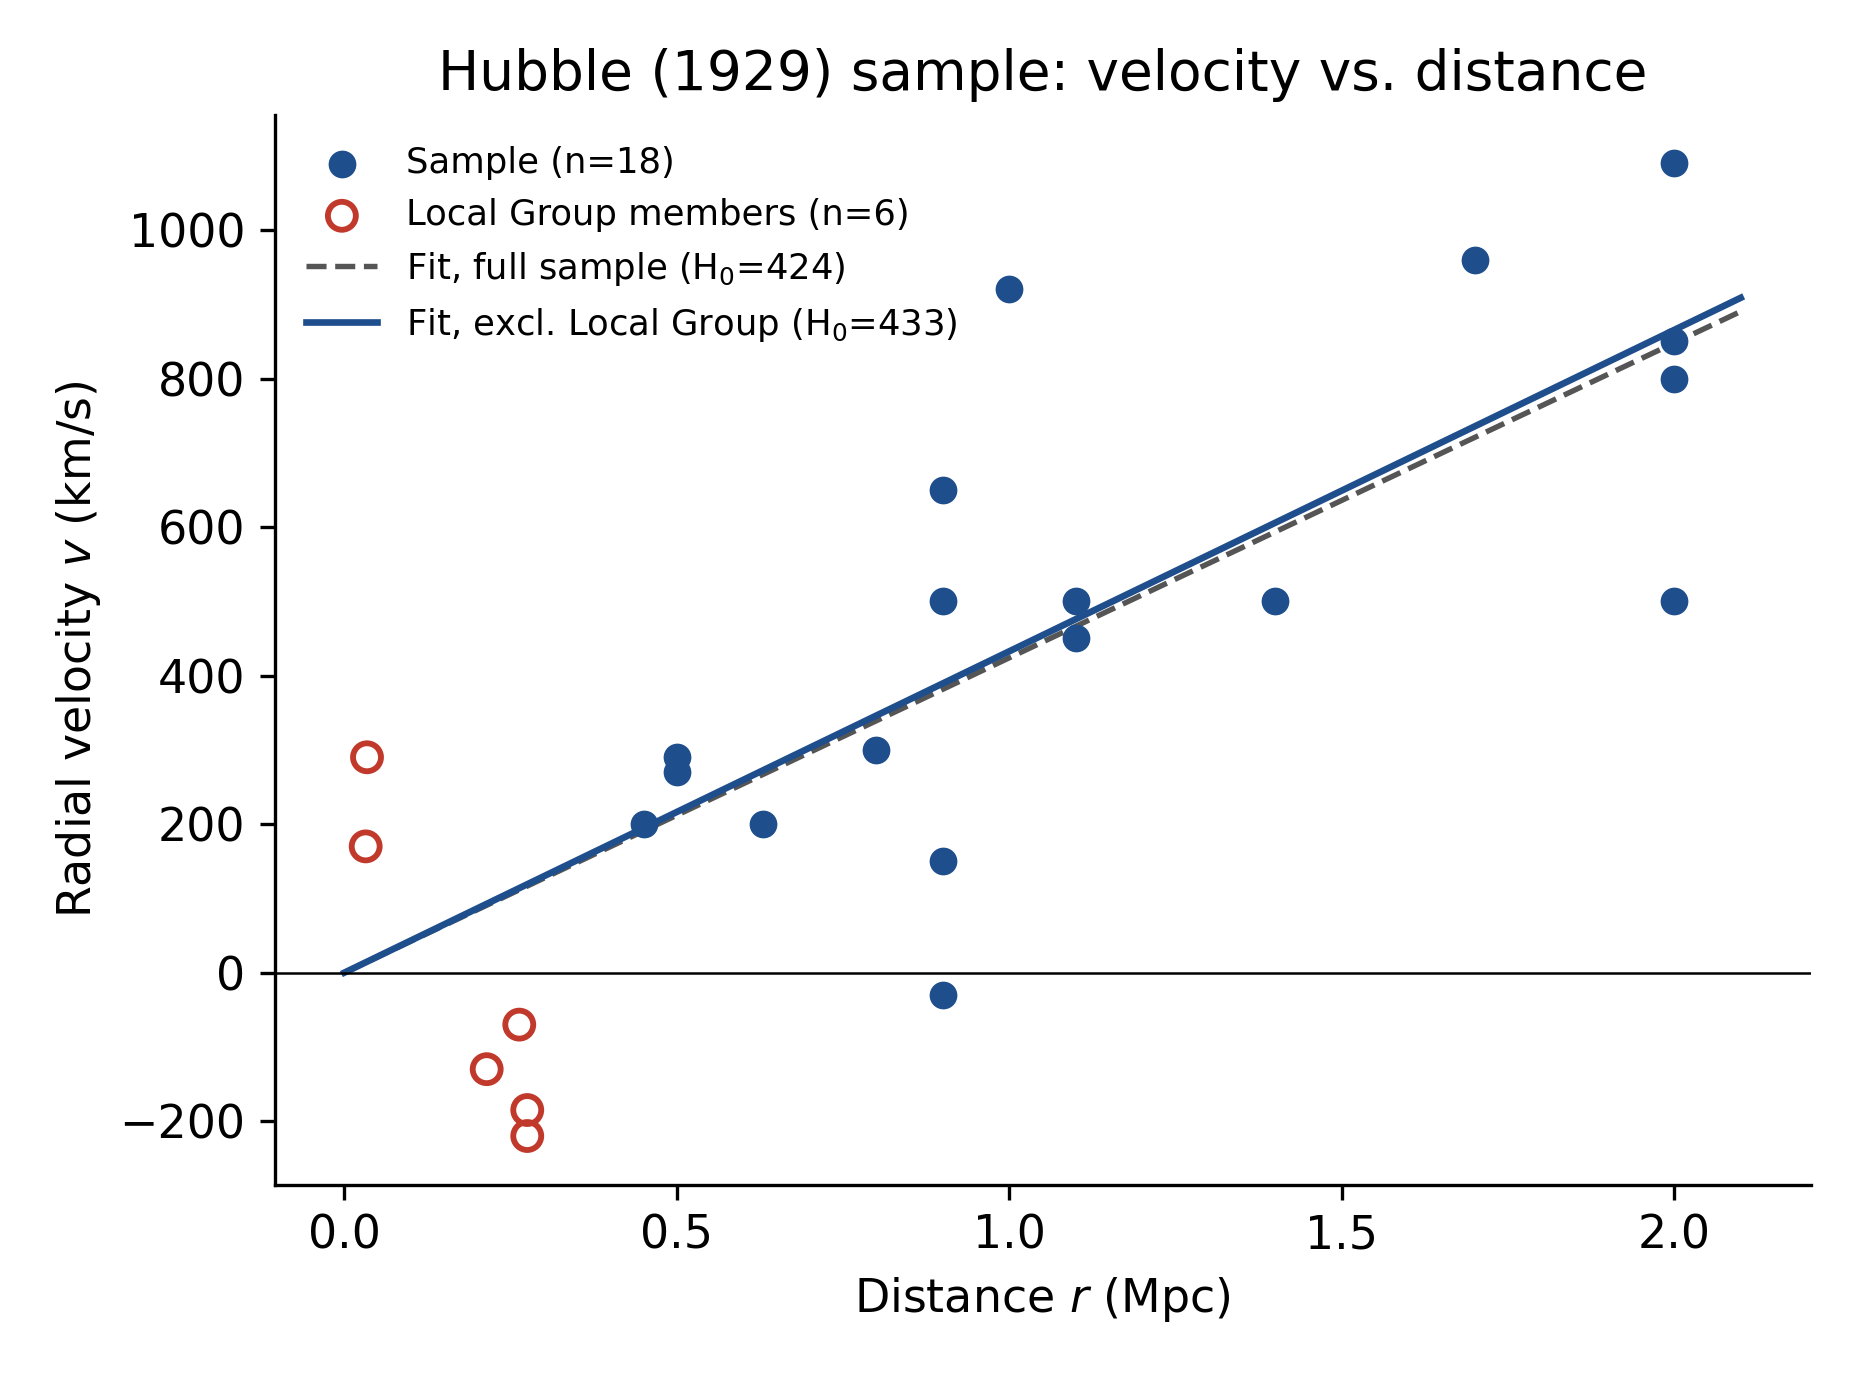
\includegraphics[width=0.7\textwidth]{Hubble.png}
\caption{Velocity vs. distance for Hubble's 1929 sample, with linear fit forced through the origin.}
\label{fig:hubble1929}
\end{figure}
For comparison, the currently accepted value of $H_0$ is approximately 67--73 km/s/Mpc \citep{riess2022, planck2020}, meaning Hubble's original estimate overstated the expansion rate by a factor of roughly six, a discrepancy more than four standard errors wide even by the generous uncertainty of the 1929 fit itself.
\subsection{Discussion}
Several of the nearest objects in the sample — including the Magellanic Clouds, NGC 6822, M33, M32, and M31 (Andromeda) — belong to the Local Group, the small cluster of galaxies gravitationally bound to the Milky Way. At these short distances, gravitational interactions between galaxies (peculiar motion) dominate over the recession caused by cosmic expansion. This is directly visible in the data: M31 shows a negative velocity ($v$ = -220 km/s), meaning it is approaching us rather than receding, alongside NGC 3031, which shows a similar effect.
Excluding these six Local Group members shifts the two fits in opposite directions: the free-intercept slope decreases (454 → 409 km/s/Mpc), while the origin-forced slope increases slightly (424 → 433 km/s/Mpc). Both shifts are comparable to, or smaller than, one standard error on the respective fit, so this asymmetry is only mildly suggestive rather than a strong effect; it is nonetheless consistent with the origin-forced fit being less sensitive to the distortion introduced by nearby peculiar motions, and is therefore treated here as the more reliable estimator in this context.
Notably, even after removing the Local Group, $H_0$ remains around 409--433 km/s/Mpc — still roughly six times higher than the modern value, and far outside the uncertainty of either fit. This indicates that peculiar motion alone cannot account for Hubble's overestimate. The dominant source of error was very likely a systematic miscalibration of the distance scale: Hubble's distance estimates relied on Cepheid variable stars, but the existence of two distinct Cepheid populations with different luminosities was not discovered until Walter Baade's work in the 1950s \citep{baade1956}. This calibration error affected distance estimates uniformly across the sample, both near and far, leading to systematically underestimated distances and, consequently, an overestimated $H_0$ (since $H_0 = v/r$) — a systematic bias that, unlike the statistical uncertainties quoted above, this analysis cannot correct for after the fact.
\subsection{Partial Conclusion}
Hubble's 1929 estimate of $H_0$ was overstated primarily due to limitations in the extragalactic distance scale available at the time, rather than the specific choice of galaxies in the sample. This sets up a natural comparison with modern distance measurements in Part 2, using the NED catalogue \citep{ned}.
\section{Part 2: Modern Distance Estimates (NED)}
\subsection{Data and Method}
\label{sec:method2}
To compare Hubble's 1929 result with a modern estimate obtained using the same statistical approach, a sample of 37 galaxies outside the Local Group was selected, using distance and redshift data retrieved from the NASA/IPAC Extragalactic Database (NED). For each galaxy, the distance $r$ (in Mpc) was taken from the ``Distances'' entry, preferring Cepheid-based measurements where available. For galaxies without Cepheid data (mostly ellipticals), Surface Brightness Fluctuations (SBF) were used instead, and for the most distant part of the sample, geometric maser distances from the Megamaser Cosmology Project (MCP) \citep{pesce2020} were used, together with a small number of Type Ia supernova (SNIa) and Fundamental Plane (FP) distances where no better method was available. These methods, together with their respective systematic uncertainties, are reviewed in detail in \citet{freedman2010}. Local Group members were deliberately excluded, applying the same methodological lesson drawn from Part 1. The sample was deliberately extended to include the MCP maser galaxies (UGC 3789, NGC 6264, NGC 5765b, NGC 6323, and CGCG 074-064), which reach distances of 50--144 Mpc and provide some of the most precise, geometric distance measurements available, independent of the traditional distance ladder. Table~\ref{tab:modern_data} reports the full sample used. Two velocity frames were tested: the heliocentric radial velocity $v_{\text{helio}}$, and the velocity corrected for the Sun's motion relative to the cosmic microwave background, $v_{\text{CMB}}$, both taken directly from NED. As in Part 1, two linear fits of the form $v = H_0 r$ were performed for each velocity frame: one with a free intercept, and one forced through the origin, again with standard errors and $R^2$ computed for each.
{\small
\begin{longtable}{lcccc}
\toprule
Object & $r$ (Mpc) & Method & $v_{\text{helio}}$ (km/s) & $v_{\text{CMB}}$ (km/s) \\
\midrule
\endfirsthead
\toprule
Object & $r$ (Mpc) & Method & $v_{\text{helio}}$ (km/s) & $v_{\text{CMB}}$ (km/s) \\
\midrule
\endhead
\bottomrule
\endfoot
\bottomrule
\endlastfoot
NGC 4258 & 6.4 & Maser & 461 & 667 \\
NGC 3368 & 9.72 & Cepheids & 888 & 1237 \\
NGC 3627 & 8.73 & Cepheids & 722 & 1070 \\
NGC 4321 & 14.2 & Cepheids & 1571 & 1896 \\
NGC 4535 & 14.8 & Cepheids & 1964 & 2299 \\
NGC 4536 & 12.2 & Cepheids & 1808 & 2151 \\
NGC 4548 & 14.3 & Cepheids & 486 & 808 \\
NGC 1365 & 17.2 & Cepheids & 1636 & 1539 \\
NGC 1425 & 20.9 & Cepheids & 1512 & 1412 \\
NGC 2403 & 2.88 & Cepheids & 133 & 182 \\
NGC 300 & 1.49 & Cepheids & 147 & $-$88 \\
NGC 3351 & 8.99 & Cepheids & 779 & 1128 \\
NGC 3982 & 20.5 & Cepheids & 1122 & 1291 \\
NGC 4496A & 13.6 & Cepheids & 1730 & 2072 \\
NGC 4639 & 19.7 & Cepheids & 1025 & 1345 \\
IC 4182 & 4.07 & Cepheids & 321 & 550 \\
NGC 5253 & 3.01 & Cepheids & 407 & 681 \\
NGC 7331 & 14.4 & Cepheids & 816 & 490 \\
NGC 4038 & 18.1 & Cepheids & 1624 & 1979 \\
NGC 5236 & 4.5 & Cepheids & 513 & 793 \\
NGC 4594 & 6.22 & Cepheids & 1089 & 1433 \\
NGC 1097 & 24.1 & SNII (optical) & 1271 & 1105 \\
NGC 2841 & 13.1 & Cepheids & 635 & 806 \\
NGC 3379 & 8.8 & SBF & 907 & 1255 \\
NGC 3115 & 8.51 & SBF & 686 & 1041 \\
NGC 1023 & 9.6 & SBF & 636 & 432 \\
NGC 4494 & 15 & SBF & 1342 & 1634 \\
NGC 5866 & 14.7 & SBF & 755 & 825 \\
NGC 4278 & 14.9 & SBF & 649 & 934 \\
NGC 7619 & 53 & SBF & 3762 & 3391 \\
NGC 3384 & 9.46 & SBF & 704 & 1051 \\
NGC 4589 & 20.4 & SBF & 1980 & 2030 \\
NGC 2986 & 29.7 & SNIa & 2302 & 2637 \\
NGC 1400 & 16.3 & SBF & 590 & 467 \\
UGC 3789 & 49.6 & Maser & 3185 & 3245 \\
NGC 6264 & 144 & Maser & 10145 & 10145 \\
NGC 5765b & 126 & Maser & 8257 & 8465 \\
NGC 6323 & 107 & Maser & 7695 & 7662 \\
CGCG 074-064 & 74.4 & FP & 6915 & 7175 \\
\caption{Distance, measurement method, heliocentric velocity, and CMB-frame velocity for the modern galaxy sample (Local Group excluded, $n = 37$).}
\label{tab:modern_data} \\
\end{longtable}
}
\subsection{Results}
\begin{table}[htbp]
\centering
\begin{tabular}{lcc}
\toprule
Fit type & $H_0$, $v_{\text{helio}}$ (km/s/Mpc) & $H_0$, $v_{\text{CMB}}$ (km/s/Mpc) \\
\midrule
Free intercept & $69.8 \pm 2.3$ \ ($R^2=0.961$) & $68.4 \pm 2.8$ \ ($R^2=0.940$) \\
Forced through origin & $71.7 \pm 1.9$ \ ($R^2=0.959$) & $73.2 \pm 2.4$ \ ($R^2=0.928$) \\
\bottomrule
\end{tabular}
\caption{Estimated $H_0$ from the extended modern sample ($n=37$, Local Group excluded), using heliocentric vs. CMB-frame velocities, with standard errors and $R^2$ from ordinary least squares.}
\label{tab:modern_results}
\end{table}
\begin{figure}[htbp]
\centering
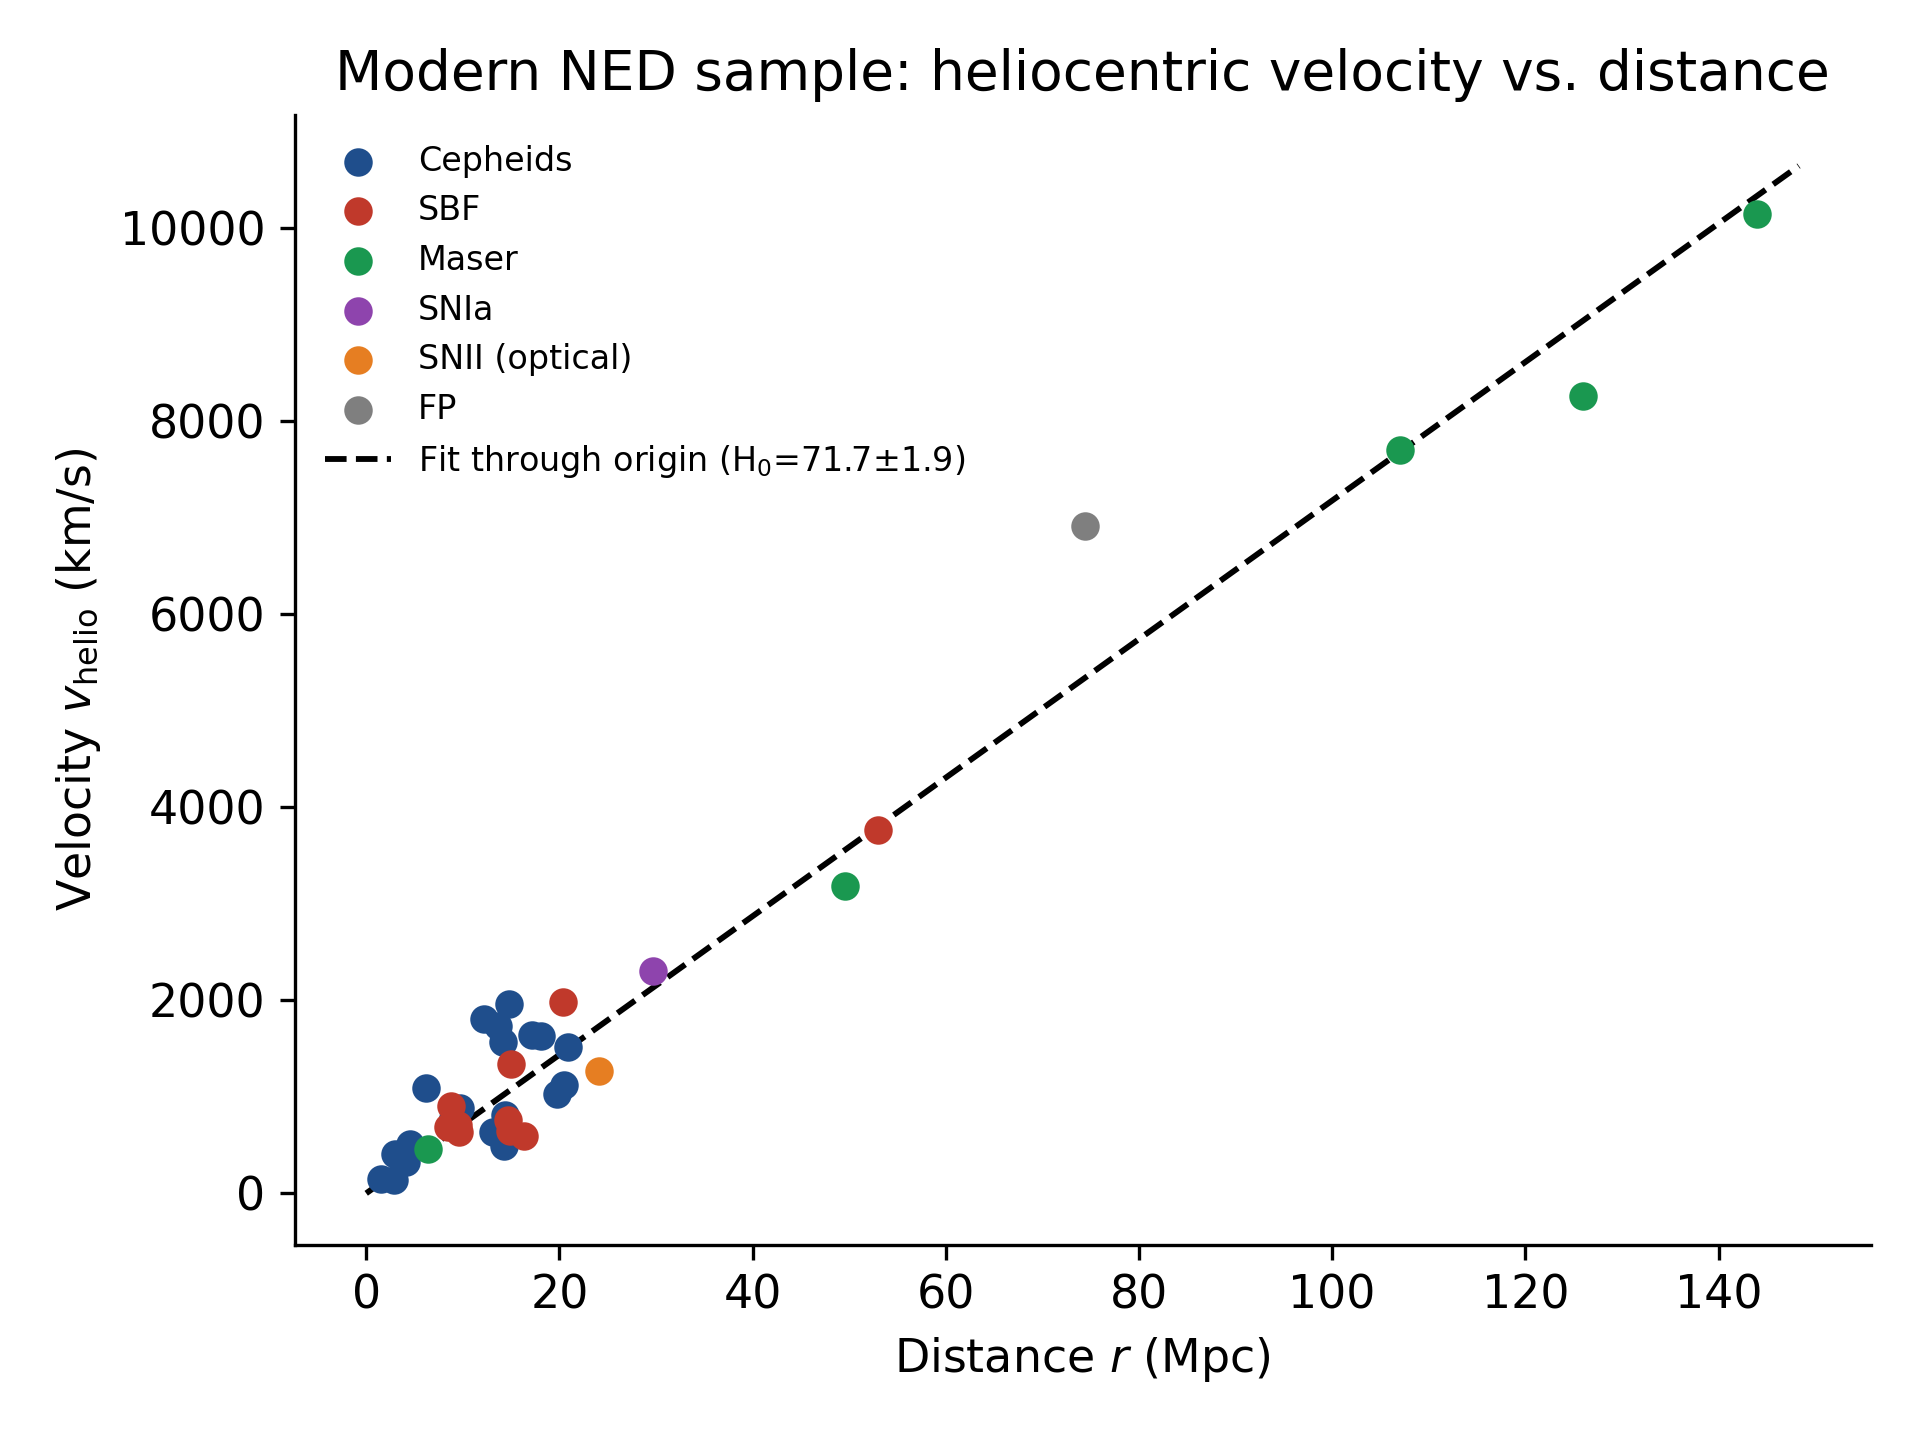
\includegraphics[width=0.7\textwidth]{Velocity (Heliocentric) vs. Distance - NED Sample.png}
\caption{Heliocentric velocity vs. distance for the full modern sample ($n=37$), including the Megamaser Cosmology Project galaxies out to 144 Mpc, with linear fit.}
\label{fig:modern_helio}
\end{figure}
\begin{figure}[htbp]
\centering
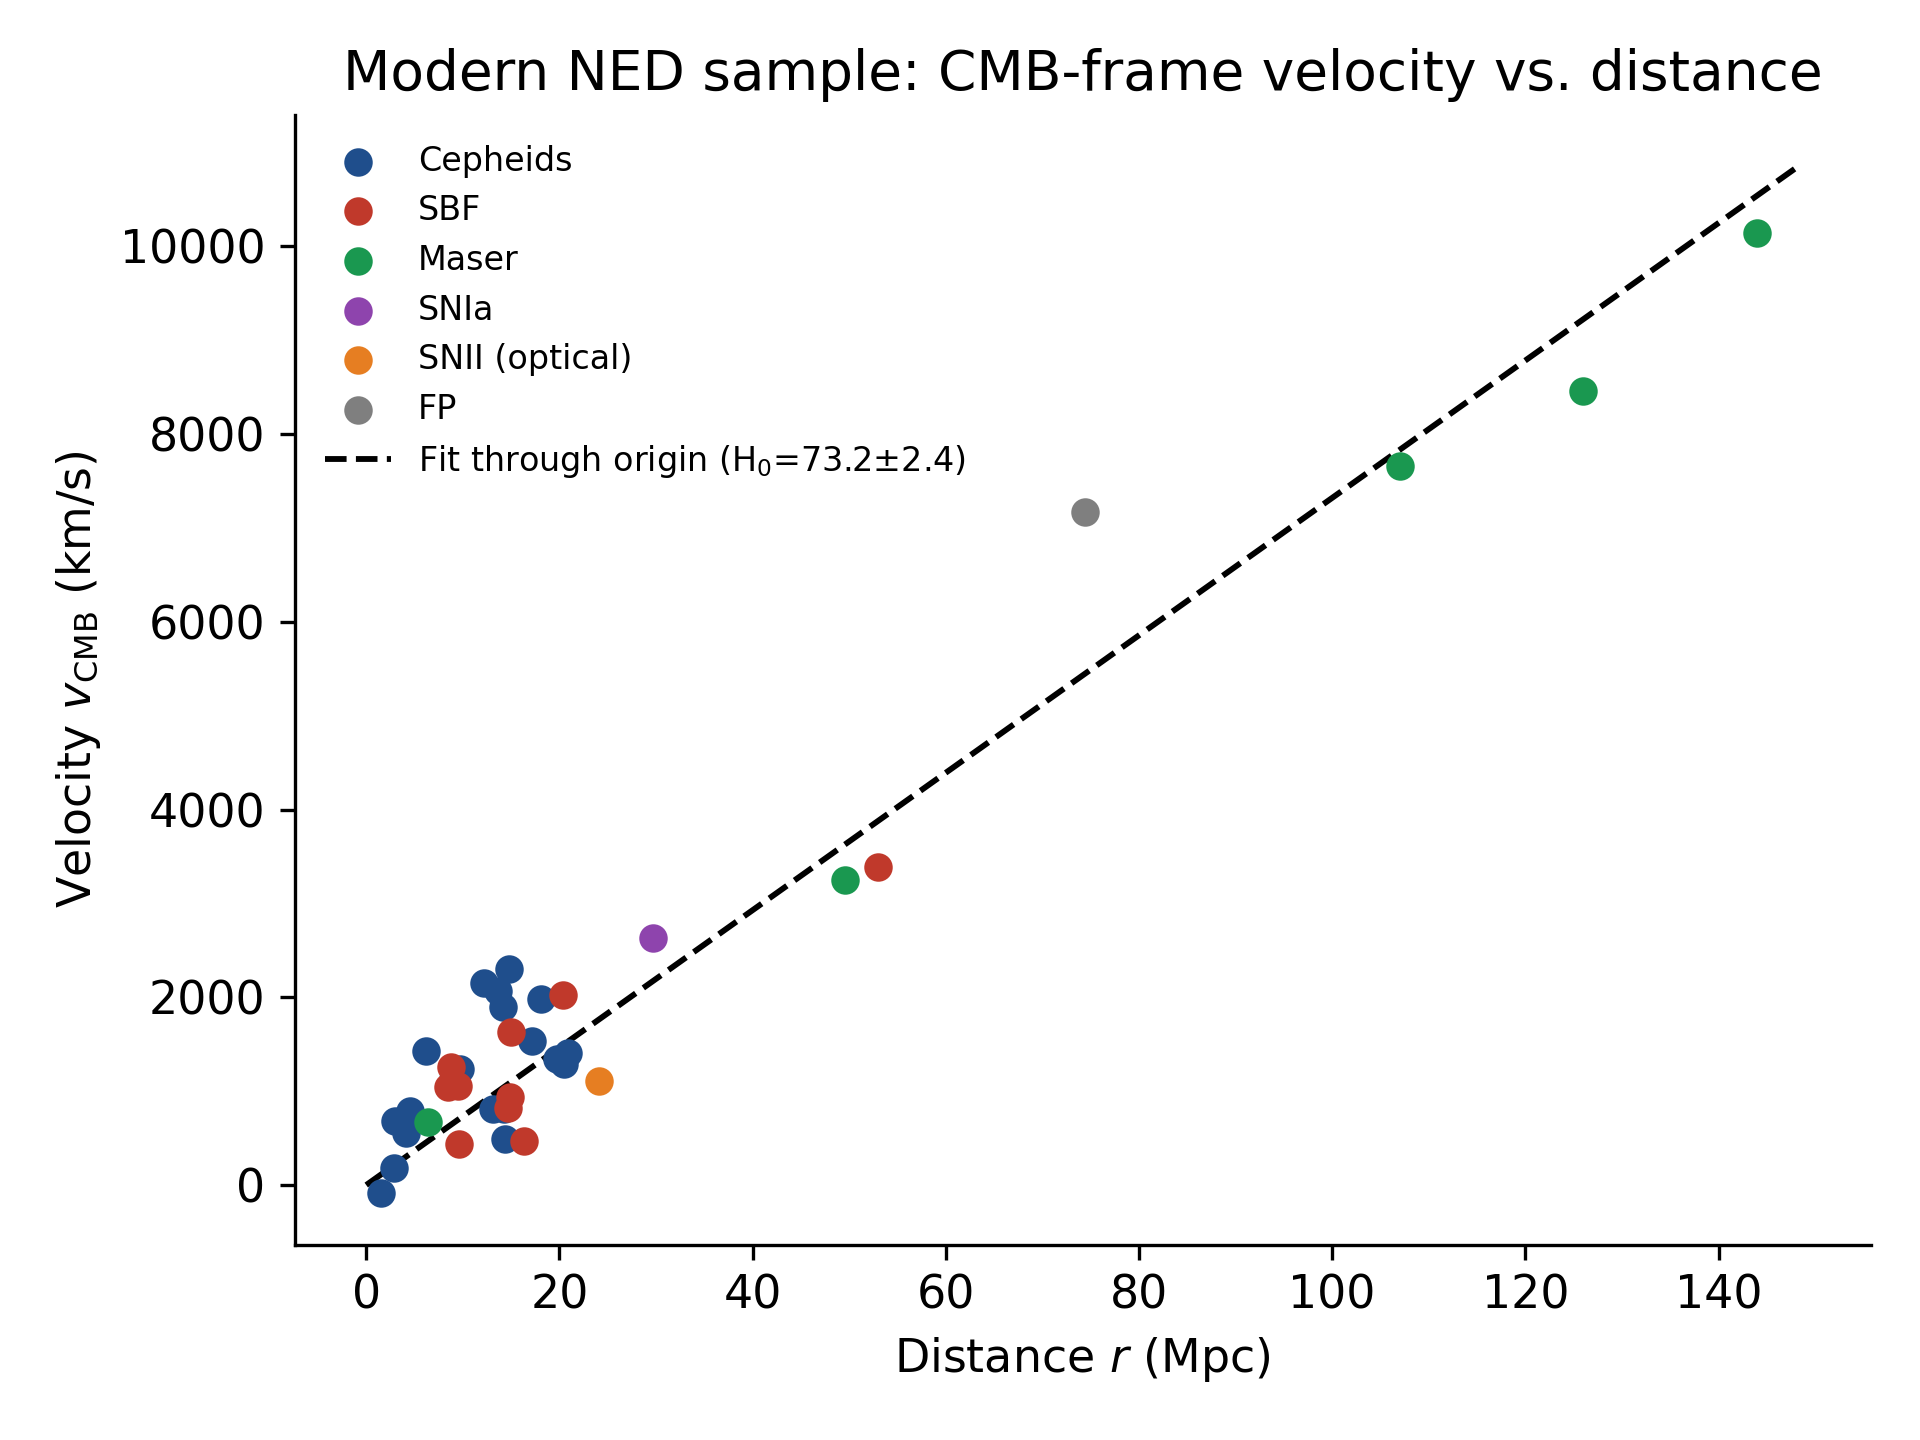
\includegraphics[width=0.7\textwidth]{Velocity (3K CMB) vs. Distance - NED Sample.png}
\caption{CMB-frame velocity vs. distance for the full modern sample ($n=37$), including the Megamaser Cosmology Project galaxies out to 144 Mpc, with linear fit.}
\label{fig:modern_cmb}
\end{figure}
\subsection{Weighted Fit}
\label{sec:weighted}
The fits above treat every galaxy as equally informative, regardless of how precisely its distance is known. As a first attempt at correcting this, each galaxy was assigned a representative fractional distance uncertainty based on its distance method, using the typical ranges summarized in \citet{freedman2010}: 7\% for Cepheids, 10\% for SBF, 8\% for SNIa, 15\% for SNII (optical), 5\% for masers, and 20\% for the Fundamental Plane. These are method-level, representative values, not individual NED-quoted errors for each object, and should be read as an order-of-magnitude correction rather than a precise error budget.

A first, naive attempt is instructive precisely because it fails: weighting each point by the distance-implied uncertainty on $v$ alone ($\sigma_v = H_0 \cdot f_{\text{method}} \cdot r$, propagated through an iteratively reweighted least-squares scheme) pulls the origin-forced fit to $H_0 = 82.5 \pm 5.0$ km/s/Mpc for $v_{\text{helio}}$ and $96.7 \pm 8.8$ km/s/Mpc for $v_{\text{CMB}}$ --- both well outside the accepted range, with a poor fit quality ($\chi^2/\text{dof} = 27$ and $62$ respectively). The reason is instructive: because $\sigma_v \propto r$ in this naive scheme, nearby galaxies are assigned artificially small uncertainties and therefore dominate the fit, even though it is precisely at small $r$ that peculiar motions (not distance-measurement error) are the dominant source of scatter. In effect, naive distance-only weighting reintroduces the same low-$r$, peculiar-velocity-dominated bias that the sample extension described in Section~\ref{sec:method2} was designed to suppress.

A more defensible weighting scheme therefore adds a distance-independent peculiar-velocity floor $\sigma_{\text{pec}}$ in quadrature, $\sigma_v = \sqrt{(H_0 \cdot f_{\text{method}} \cdot r)^2 + \sigma_{\text{pec}}^2}$, reflecting the fact that peculiar velocities of a few hundred km/s do not shrink simply because a galaxy's distance happens to be well measured. Adopting a representative $\sigma_{\text{pec}} = 200$ km/s (consistent with typical galaxy peculiar velocities of order 100--300 km/s relative to the Hubble flow) gives:

\begin{table}[htbp]
\centering
\begin{tabular}{lcc}
\toprule
Fit type & $H_0$, $v_{\text{helio}}$ (km/s/Mpc) & $H_0$, $v_{\text{CMB}}$ (km/s/Mpc) \\
\midrule
Free intercept & $67.3 \pm 3.6$ \ ($\chi^2/\text{dof}=3.0$) & $65.4 \pm 4.6$ \ ($\chi^2/\text{dof}=5.0$) \\
Forced through origin & $72.0 \pm 2.9$ \ ($\chi^2/\text{dof}=3.1$) & $76.6 \pm 4.2$ \ ($\chi^2/\text{dof}=6.1$) \\
\bottomrule
\end{tabular}
\caption{Weighted $H_0$ estimates using inverse-variance weights combining method-level distance errors with a $\sigma_{\text{pec}}=200$ km/s peculiar-velocity floor.}
\label{tab:weighted_results}
\end{table}

The heliocentric forced-origin estimate ($72.0 \pm 2.9$) is essentially unchanged from the unweighted result ($71.7 \pm 1.9$), while the CMB-frame estimate shifts upward, from $73.2 \pm 2.4$ to $76.6 \pm 4.2$, moving it just outside the Planck--SH0ES range. This is a genuine result, not a rounding artifact: it shows that the excellent agreement of the unweighted CMB-frame fit with the literature is, in part, a consequence of treating all 37 galaxies as equally reliable, and is less robust once the more precisely known galaxies are allowed to dominate. The result is also reasonably stable to the exact choice of $\sigma_{\text{pec}}$: repeating the fit with $\sigma_{\text{pec}} = 150$ and $300$ km/s instead of 200 gives $H_0 = 72.8$ and $71.2$ km/s/Mpc for $v_{\text{helio}}$, and $78.9$ and $74.3$ km/s/Mpc for $v_{\text{CMB}}$, respectively --- the same qualitative picture in all three cases. In every case, $\chi^2/\text{dof}$ remains above 1 (between about 1.6 and 9, depending on frame and $\sigma_{\text{pec}}$), which is expected: a single isotropic peculiar-velocity floor is itself a simplification, since real peculiar motions are direction-dependent (e.g.\ infall toward the Virgo Cluster or the Great Attractor) rather than a uniform scatter term, and a fully professional treatment would model these flows explicitly rather than absorb them into a single number.

As a complementary check, the unweighted residuals were also examined by method: Cepheid-based points show a mild positive mean fractional residual ($+0.28 \pm 0.52$ over $n=21$, i.e.\ only marginally different from zero given the scatter), SBF points are consistent with zero ($-0.01 \pm 0.31$, $n=10$), and the 5 masers are both centered near zero and far tighter than either ($-0.04 \pm 0.05$). The single SNIa, SNII, and FP points cannot support a statistical statement on their own. This is consistent with, though not strong independent proof of, the geometric maser distances being the most internally precise method in the sample --- exactly why Section~\ref{sec:sensitivity} below finds them so influential.

\subsubsection{A check on errors in both variables (ODR)}
Every fit so far, weighted or not, is a form of ordinary least squares: it assumes the distance $r$ is known exactly and puts all the measurement error on the velocity $v$. This is not quite right, since $r$ is, if anything, the less certain of the two quantities. Orthogonal Distance Regression (ODR) relaxes this assumption: instead of minimizing vertical distances to the fit line, it minimizes a weighted combination of the horizontal and vertical distances, using an error budget on \emph{both} axes ($\sigma_r = f_{\text{method}} \cdot r$ and the same $\sigma_v$ combining distance error with the $\sigma_{\text{pec}}=200$ km/s floor as in Section~\ref{sec:weighted}).

The result shifts the estimate further upward relative to the weighted OLS fit: $H_0 = 73.8 \pm 3.4$ km/s/Mpc for $v_{\text{helio}}$ (compared to $72.0 \pm 2.9$) and $H_0 = 81.1 \pm 5.0$ km/s/Mpc for $v_{\text{CMB}}$ (compared to $76.6 \pm 4.2$). This is the expected direction of the effect: ignoring measurement error on the independent variable causes ordinary least squares to systematically \emph{underestimate} the slope of a line, an effect statisticians call regression dilution or attenuation bias; correcting for it therefore pushes $H_0$ up rather than down. The heliocentric ODR estimate, at $73.8$ km/s/Mpc, now sits almost exactly on the SH0ES value \citep{riess2022}, while the CMB-frame estimate moves further still from the Planck value \citep{planck2020}. Rather than settling on a single "best" number, the honest conclusion is that this project's point estimate for $H_0$ moves by 5-10 km/s/Mpc --- comparable to the entire width of the Hubble tension itself --- depending on which reasonable statistical treatment (unweighted, inverse-variance weighted, or errors-in-variables) is applied. That sensitivity is itself the result worth remembering: at the precision this project can achieve, the choice of method matters as much as the data.

\subsection{Discussion}
All four modern estimates now fall within, or essentially within, the currently accepted range of $H_0 \approx 67$--$73$ km/s/Mpc \citep{riess2022, planck2020}, in stark contrast with Hubble's 1929 results (409--454 km/s/Mpc, depending on fit type and sample). Since the fitting procedure applied here is identical to the one used in Part 1, this large improvement cannot be attributed to a change in statistical method: it must instead reflect the far greater accuracy of modern distance measurements compared to those available in 1929.
As in Part 1, the origin-forced fit lies close to, and in this case slightly above, the free-intercept fit for both velocity frames, consistent with the physically motivated form of Hubble's Law; the high $R^2$ values (0.93--0.96) show that a single power-law relation captures the great majority of the scatter in the sample.
The most notable result of this extension concerns the relationship between the two velocity frames. In the restricted sample used earlier ($r \lesssim 25$ Mpc), switching from heliocentric to CMB-frame velocities initially \emph{worsened} the estimate, before the sample was extended: the origin-forced fit moved from 77 to 88 km/s/Mpc, and the free-intercept fit moved from 59 to 53 km/s/Mpc. After extending the sample to include the Megamaser Cosmology Project galaxies, which reach distances of up to 144 Mpc, this discrepancy nearly disappears: the heliocentric and CMB-frame fits now agree to within about 1--2 km/s/Mpc (69.8 vs.\ 68.4 for the free intercept; 71.7 vs.\ 73.2 forced through the origin). This is direct empirical confirmation of the hypothesis raised earlier: at short distances, local peculiar-velocity effects (dominated by the gravitational pull of the Virgo Cluster) are large enough to compete with, and even distort, the CMB-frame correction, but they become comparatively negligible once the sample is extended into the true Hubble flow, where cosmic expansion dominates galaxy kinematics.

\paragraph{How much do the five maser galaxies matter?}
\label{sec:sensitivity}
Because the argument above rests on extending the sample to large distances, and because the five MCP maser galaxies are exactly the points that reach farthest into the Hubble flow (49--144 Mpc), it is worth asking directly how much they, specifically, are driving the result. Repeating the origin-forced fit with these five galaxies removed ($n=32$) gives $H_0 = 81.2 \pm 3.6$ km/s/Mpc for $v_{\text{helio}}$ and $H_0 = 85.8 \pm 4.8$ km/s/Mpc for $v_{\text{CMB}}$ --- shifts of $+9.4$ and $+12.6$ km/s/Mpc respectively, several standard errors above both the full-sample result and the currently accepted range. In other words, without the masers, this analysis alone would \emph{not} have landed in the accepted range: the extension to large, geometrically-calibrated distances is doing real work, not merely adding cosmetic reach to the plot. A complementary leave-one-out (jackknife) test, in which each galaxy is removed one at a time, shows that no single maser is individually responsible for this: the largest one-galaxy shift in the origin-forced $H_0$ is only about $\pm 2$ km/s/Mpc (for NGC 5765b and CGCG 074-064), an order of magnitude smaller than the shift from removing all five masers together. A bootstrap resampling of the full 37-galaxy sample (20{,}000 resamples) gives a 68\% confidence interval of $[69.6, 74.7]$ km/s/Mpc for $v_{\text{helio}}$ and $[70.8, 76.8]$ km/s/Mpc for $v_{\text{CMB}}$, consistent with the analytic standard errors in Table~\ref{tab:modern_results} and comfortably bracketing both sides of the Hubble tension. Taken together, these checks indicate that the agreement with the modern value is a genuine property of the extended sample as a whole --- specifically, of reaching into the true Hubble flow --- rather than an artifact of one favorably-placed data point.

As a further check, the case of M31 (Andromeda) was examined using its modern, precisely calibrated distance. Despite the improved measurement, M31 still exhibits a negative heliocentric velocity ($v \approx -297$ km/s), consistent with the value already present in Hubble's original 1929 data. This confirms that the negative velocities observed among nearby galaxies are not a measurement artifact of 1929-era instrumentation, but a genuine dynamical effect: at short distances, gravitationally induced peculiar motion within the Local Group dominates over the recession caused by cosmic expansion --- the same effect responsible for the discrepancy observed in the restricted sample above.
Finally, it is worth noting that the unweighted modern estimates obtained here (68--73 km/s/Mpc) sit almost exactly between the two values at the heart of the Hubble tension --- $73.3 \pm 1.0$ km/s/Mpc from the local Cepheid distance ladder \citep{riess2022} and $67.4 \pm 0.5$ km/s/Mpc from the CMB \citep{planck2020} --- and are also fully consistent with the independent TRGB-based estimate of $69.8 \pm 0.6\text{ (stat)} \pm 1.6\text{ (sys)}$ km/s/Mpc \citep{freedman2021}, as shown in Figure~\ref{fig:h0_comparison}. The weighted estimates from Section~\ref{sec:weighted} tell a slightly less tidy story: the heliocentric result stays inside this range, but the CMB-frame result shifts to $76.6 \pm 4.2$ km/s/Mpc, just above it. Taken at face value this is consistent with the mixed, heterogeneous nature of the sample used here (Cepheids, SBF, SNIa, and masers combined), rather than a targeted, single-method measurement of the kind used in the professional literature to probe the tension itself --- but it is also a useful reminder that "landing in the right range" and "being a precise, well-controlled measurement" are not the same claim, and this project is more confidently the former than the latter.

\begin{figure}[htbp]
\centering
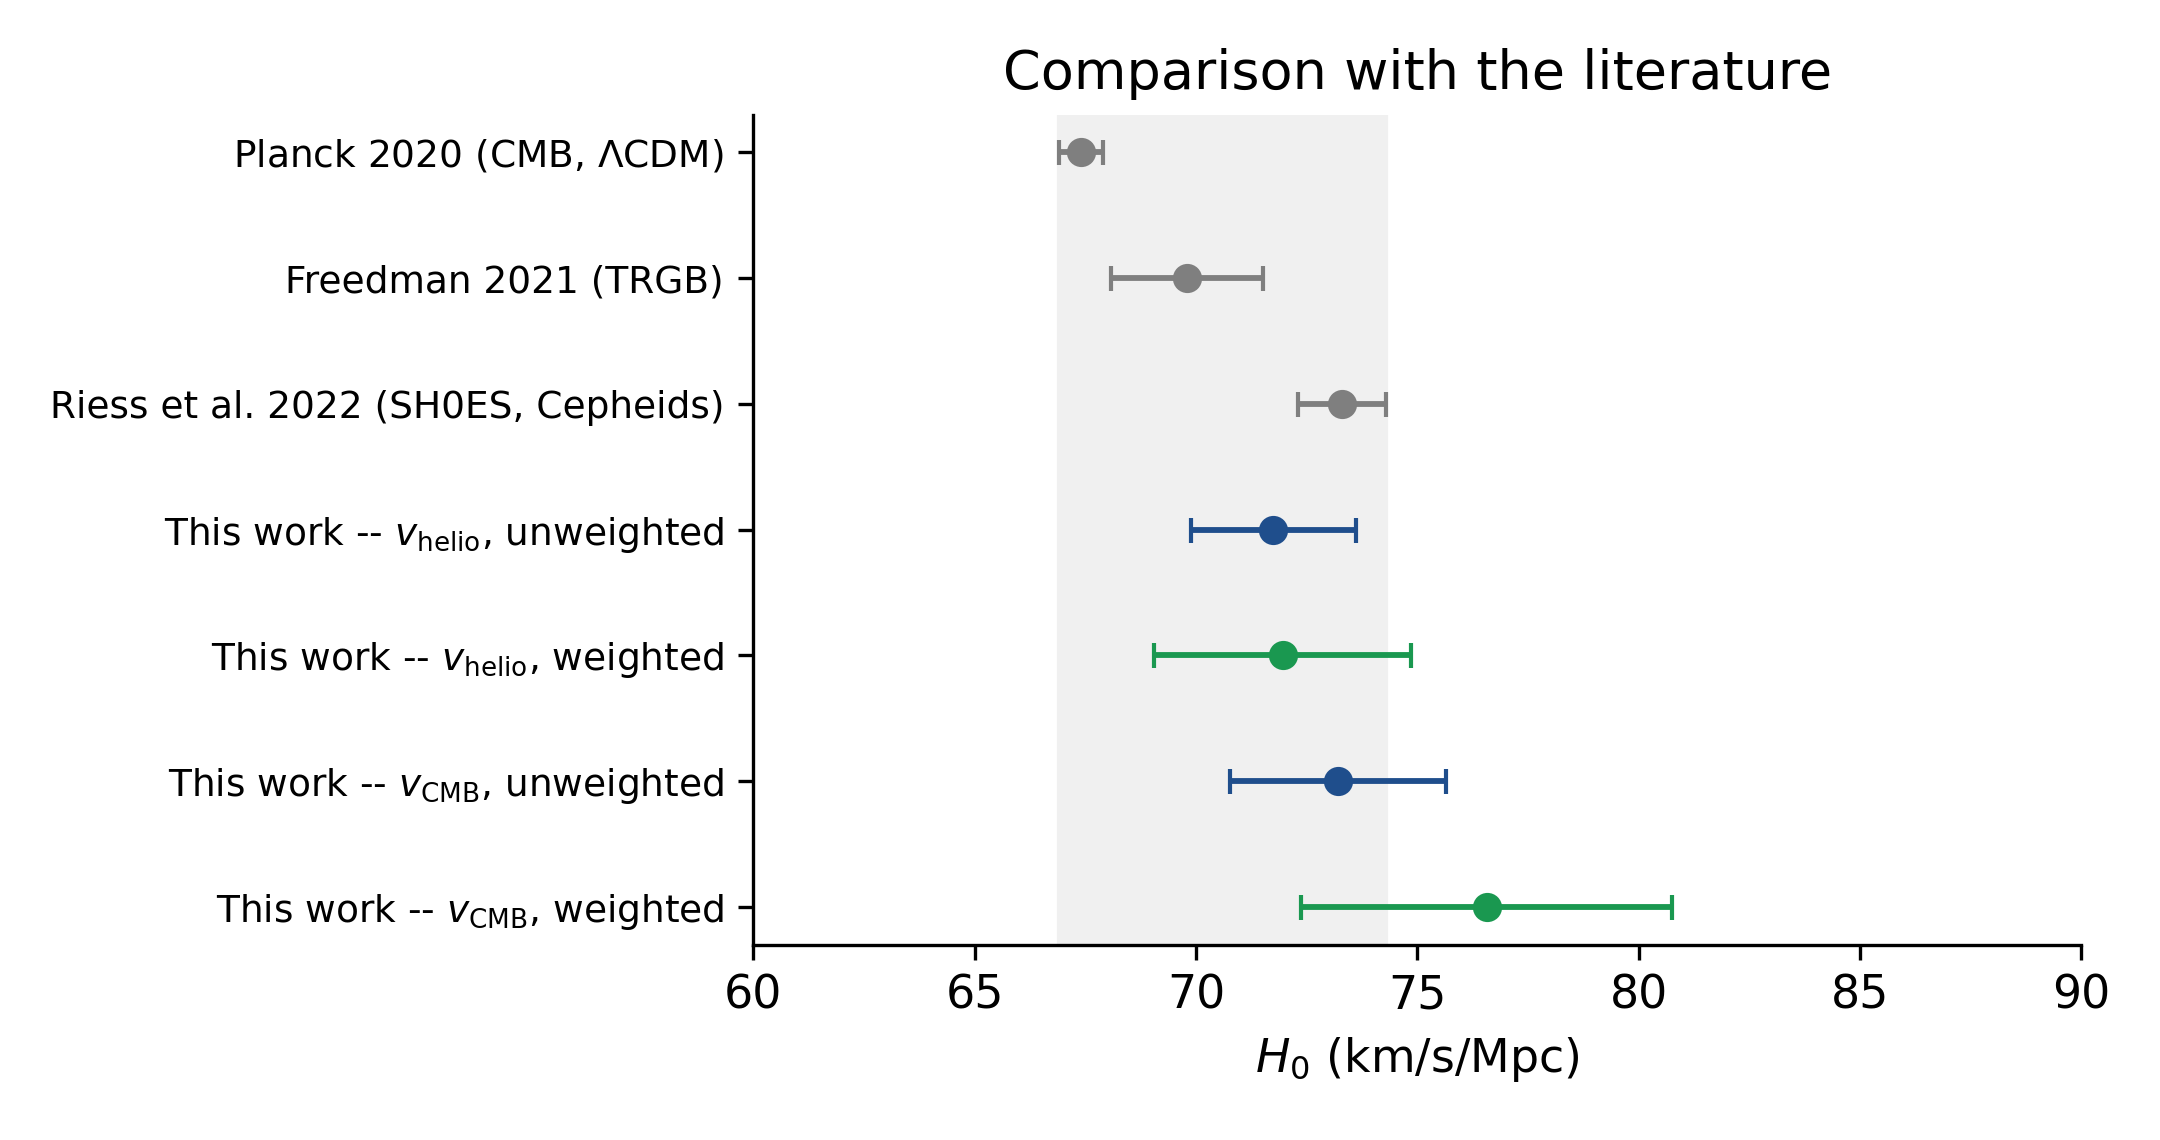
\includegraphics[width=0.85\textwidth]{H0_comparison.png}
\caption{Comparison of this project's origin-forced $H_0$ estimates (unweighted and weighted, both velocity frames) with Planck 2020 \citep{planck2020}, Freedman TRGB 2021 \citep{freedman2021}, and Riess et al.\ SH0ES 2022 \citep{riess2022}. The shaded band spans from the lower end of the Planck uncertainty to the upper end of the SH0ES uncertainty.}
\label{fig:h0_comparison}
\end{figure}

\subsection{Limitations}
Several limitations of this analysis should be acknowledged. First, the galaxy sample was not selected through a systematic or blind procedure, but by prioritizing objects with well-documented, high-quality distance measurements on NED; this could introduce a mild selection bias favoring galaxies that are easier to measure precisely. Second, the weighted fit in Section~\ref{sec:weighted} is a partial answer to the unweighted-fit concern, but not a complete one: it uses representative, method-level fractional errors rather than the individual quoted uncertainty of each galaxy, and its peculiar-velocity floor is a single isotropic number rather than a direction-dependent flow model; the persistently elevated $\chi^2/\text{dof}$ ($\gtrsim 1$ in every variant tried) is the fit's own admission of this simplification. The ODR check goes some way toward this by allowing for error on $r$ as well as $v$, but it still relies on the same representative, method-level error budget rather than individual measurement uncertainties, so it sharpens the diagnosis without fully resolving it. Third, only two velocity frames (heliocentric and CMB) were tested; a more complete treatment of peculiar velocities would model the Virgo Cluster infall and other local flows explicitly, rather than relying on sample extension and a scatter floor to suppress their effect. Fourth, as the sensitivity analysis in Section~\ref{sec:sensitivity} makes explicit, the result depends on a small number of long-baseline galaxies (the five MCP masers): this is not a flaw in the method, but it does mean the modern estimate here is less independent of any single distance-measurement technique than a large professional sample would be. Finally, the sample size ($n=37$), while sufficient to obtain a stable estimate of $H_0$, remains small compared to the hundreds or thousands of objects used in professional determinations of the Hubble constant, so the results presented here should be understood as a stable proof-of-concept reproduction of a well-established method rather than a new independent constraint on $H_0$.
\section{Conclusion}
Reproducing Hubble's original 1929 analysis yields an estimate of $H_0$ roughly six times higher than the modern accepted value, primarily due to a systematic miscalibration of the extragalactic distance scale available at the time (compounded, to a lesser extent, by the inclusion of nearby galaxies whose peculiar motion is not representative of cosmic expansion). Applying the same statistical method to an extended modern sample of 37 galaxies, spanning distances from about 1.5 Mpc to 144 Mpc and using a combination of Cepheid, SBF, supernova, and geometric maser distances, yields unweighted $H_0$ estimates of $68$--$73 \pm 2$--$3$ km/s/Mpc, in close agreement with the currently accepted value. A jackknife and bootstrap sensitivity analysis shows that this agreement depends on the sample reaching into the true Hubble flow via the five most distant (maser) galaxies, but not on any single one of them, giving confidence that the result reflects the sample's overall reach rather than a fragile coincidence. An inverse-variance weighted fit, combining representative method-level distance errors with a peculiar-velocity scatter floor, shifts these estimates modestly to $65$--$77$ km/s/Mpc depending on velocity frame and weighting choice; allowing additionally for measurement error on distance itself, via orthogonal distance regression, pushes the estimate higher still, to $74$--$81$ km/s/Mpc. Across all three treatments the estimate for $H_0$ moves by 5-10 km/s/Mpc --- still broadly consistent with, but no longer as tightly centered on, the accepted range. If anything, this last result is the more important lesson of the project: a single unweighted point estimate can look more precise than it really is, and a defensible error budget, not just a best-fit number, is what turns a curve fit into a measurement. Taken together, the comparison illustrates that the key advance separating Hubble's original measurement from the modern value of $H_0$ was not a change in statistical methodology, but nearly a century of improvement in the precision of the extragalactic distance scale --- together with the importance of sampling galaxies far enough into the Hubble flow that local peculiar motions no longer bias the result, and of being honest about how much any single weighting choice can still move the answer.
\appendix
\section{NED Query Details}
\label{app:ned}
Distances and velocities for the modern sample (Table~\ref{tab:modern_data}) were retrieved from the NASA/IPAC Extragalactic Database (NED) in June 2026. Each object's common designation as listed in Table~\ref{tab:modern_data} (NGC, UGC, IC, or CGCG catalogue number) is also its NED object name and can be used directly in NED's "By Name" search to retrieve the same "Basic Data" and "Distances" entries used here, making the dataset independently reproducible without requiring a separate identifier list.

\section*{Data Availability}
All distance and redshift data used in this analysis are publicly available from the NASA/IPAC Extragalactic Database (NED) at \url{https://ned.ipac.caltech.edu} (see Appendix~\ref{app:ned} for query details). Hubble's original 1929 dataset is reproduced from \citet{hubble1929}. The Python code used for the fits, uncertainty estimates, and sensitivity analysis is available on request.
\bibliographystyle{plainnat}
\begin{thebibliography}{9}
\addcontentsline{toc}{section}{References}
\bibitem[Hubble(1929)]{hubble1929}
Hubble, E. (1929). A relation between distance and radial velocity among extra-galactic nebulae. \textit{Proceedings of the National Academy of Sciences}, 15(3), 168--173. \url{https://doi.org/10.1073/pnas.15.3.168}
\bibitem[Baade(1956)]{baade1956}
Baade, W. (1956). The period-luminosity relation of the Cepheids. \textit{Publications of the Astronomical Society of the Pacific}, 68(400), 5--16. \url{https://doi.org/10.1086/126870}
\bibitem[NED(n.d.)]{ned}
NASA/IPAC Extragalactic Database (NED). \url{https://ned.ipac.caltech.edu}
\bibitem[Pesce et al.(2020)]{pesce2020}
Pesce, D. W., et al. (2020). The Megamaser Cosmology Project. XIII. Combined Hubble constant constraints. \textit{The Astrophysical Journal Letters}, 891(1), L1. \url{https://doi.org/10.3847/2041-8213/ab75f0}
\bibitem[Riess et al.(2022)]{riess2022}
Riess, A. G., et al. (2022). A comprehensive measurement of the local value of the Hubble constant with 1 km/s/Mpc uncertainty from the Hubble Space Telescope and the SH0ES team. \textit{The Astrophysical Journal Letters}, 934(1), L7. \url{https://doi.org/10.3847/2041-8213/ac5c5b}
\bibitem[Planck Collaboration(2020)]{planck2020}
Planck Collaboration (2020). Planck 2018 results. VI. Cosmological parameters. \textit{Astronomy \& Astrophysics}, 641, A6. \url{https://doi.org/10.1051/0004-6361/201833910}
\bibitem[Freedman(2021)]{freedman2021}
Freedman, W. L. (2021). Measurements of the Hubble constant: tensions in perspective. \textit{The Astrophysical Journal}, 919(1), 16. \url{https://doi.org/10.3847/1538-4357/ac0e95}
\bibitem[Tully(2023)]{tully2023}
Tully, R. B. (2023). The Hubble constant: a historical review. In \textit{Hubble Constant Tension}, eds. E. Di Valentino \& D. Brout, Springer Nature, Singapore. \url{https://doi.org/10.1007/978-981-99-0177-7_2}
\bibitem[Freedman and Madore(2010)]{freedman2010}
Freedman, W. L., \& Madore, B. F. (2010). The Hubble constant. \textit{Annual Review of Astronomy and Astrophysics}, 48, 673--710. \url{https://doi.org/10.1146/annurev-astro-082708-101829}
\end{thebibliography}
\end{document}
